% Source: http://tex.stackexchange.com/a/5374/23931
\documentclass{article}
\usepackage[T1]{fontenc}
\usepackage[utf8]{inputenc}
\usepackage[margin=1in]{geometry}
\usepackage{amsmath}
\usepackage{graphicx}

\newcommand{\HRule}{\rule{\linewidth}{0.5mm}}
\newcommand{\Hrule}{\rule{\linewidth}{0.3mm}}

\makeatletter% since there's an at-sign (@) in the command name
\renewcommand{\@maketitle}{%
  \parindent=0pt% don't indent paragraphs in the title block
  \centering
  {\Large \bfseries\textsc{\@title}}
  \HRule\par%
  \textit{\@author \hfill \@date}
  \par
}
\makeatother% resets the meaning of the at-sign (@)

\title{Plan of Study}
\author{Clayton W. Seitz}
\date{\today}

\begin{document}
  \maketitle% prints the title block
\vspace{0.4in}

\section{Introduction}

The central dogma of molecular biology has recently stimulated the development of a rich set of computational techniques for cellular phenotyping at the molecular scale. The intracellular environment harbors a diverse set of biomolecules which undergo complex interactions in order to carry out cellular functions. Classical biological techniques have yielded great insights into biochemical and biophysical mechanisms of these interactions; however, the development of even simple models of the interaction scheme of DNA, RNA, and protein remains a challenge. This barrier in turn precludes the abstraction of fundamental interactions to the scale of the phenotype. At the same time, recent advances in single-cell sequencing and multiplexed fluorescent labeling of nucleic acids and proteins present a practical top-down route to this abstraction, if complemented by the appropriate analysis paradigm. Indeed, high-throughput variants of these methods e.g., genome wide or transcriptome wide analyses,  output data volumes that have enabled discovery-driven research. This has important implications for both fundamental biological research as well as the discovery of the molecular drivers of disease states.

One of the most common applications of machine learning in molecular biology has been the use of supervised learning to learn a mapping from a high-dimensional dataset to a target variable of interest. This amounts to learning a conditional probability distribution $p(y|\mathbf{x})$, where $x$ is, in general, a high-dimensional variable such as a gene expression profile while $y$ is a target variable such as the cellular phenotype. This technique falls into a broader class of \emph{dicriminative} learning algorithms such as random forests, support vector machines, and multi-layer perceptrons. Such algorithms exploit the structure of $\mathbf{x}$ to learn its relationship to $y$ and are a preferred method when we are not directly concerned with the statistical structure of the input covariates $\mathbf{x}$. On the other hand, occasionally we are interested in the statistics of $\mathbf{x}$ itself, as is the case in protein design, analyzing genomic mutations, and dissecting transcriptional variability between single cells. In supervised generative learning, we try to explicity learn the joint distribution which produced that data - a task which is generally a more difficult task than discriminative learning. Overcoming the barrier to generative modeling carries significant benefits; fitting complete multivariate distributions goes beyond correlation-based or clustering approaches as it permits the discovery of partial correlations, outlier detection, as well as sampling based inference. 

When modeling $p(\mathbf{x})$, the dimension $N$ of $\mathbf{x}$ is often very large, as is the case when $\mathbf{x}$ is an image or a genome wide expression profile. Typically, we are given a finite number of empirical observations of $\mathbf{x}$ with the hope of constructing $p(\mathbf{x})$ from those observations. In high dimensions, the volume of the state space grows exponentially in the number of dimensions while we generally do not have a comparable number of training examples to accurately ``populate'' this volume. Even if we did have a sufficient number of samples to obtain a good estimate of $p(\mathbf{x})$, simply \emph{counting} the number of times each $\mathbf{x}$ to construction $p(\mathbf{x})$ is generally intractable. This can be seen from the fact that if $\mathbf{x_{i}}\in \Omega$ where $\Omega$ is the state space of each element of $\mathbf{x}$, normalizing the counts requires an summation over $|\Omega|^{N}$ possible states. This issue arises in many contexts, for example Bayesian inference and a large class of problems in statistical physics. 

Using deep networks to represent $p(\mathbf{x})$ is an active area of research, as deep networks are well-known to be flexible and expressive in modeling high-dimensional data. Two state of the art methods: variational autoencoders (VAEs) and generative adversarial networks (GANs) implement generative models as deep networks. In biological research, GANs have fewer significant contributions compared to VAEs, partially because that they do not provide an immediate way of tracing back the representation of each observation in the latent space (Lopez 2020).

In generative modelings, there is often a trade-off between model complexity and interpretability. Models that use neural networks, which perform non-linear operations, are often difficult to interpret.


\begin{figure}
\centering
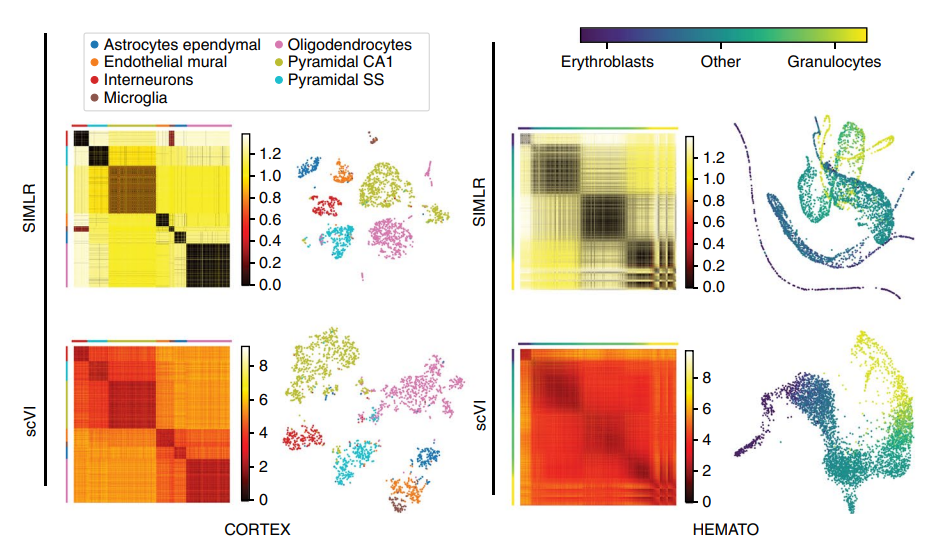
\includegraphics[width=0.7\textwidth]{force}
\caption{\textbf{Variational autoencoder architecture} Taken from Lopez 2020 in EMBO}
\end{figure}





\section{Statistical physics of deep learning}



In classical gradient descent, we attempt to find a global minimum a generally non-convex function $\mathcal{L}(\Phi)$ by compute the gradient $\nabla_{\Phi} \mathcal{L}$ with respect to the parameters or ``position vector'' $\Phi$. By iteratively computing the gradient and updating the parameters, we can arrive at a local minimum of $\mathcal{L}$. This method works well when we can explicitly evaluate $\nabla_{\Phi} \mathcal{L}$ but this is rarely the case in real-world optimization problems. We typically can only \emph{estimate} the value of the loss $\mathcal{L}(\Phi)$ based on a batch of training examples. Those training examples are sampled from $p(\mathbf{x})$ at random, which means the evolution of the parameters $\Phi$ is a stochastic process. In this scenario, conventional gradient descent becomes stochastic gradient descent or SGD. 

\begin{equation*}
\frac{d\Phi}{dt} = - \eta \hat{g}
\end{equation*}

which is analogous to a ``velocity''. It follows that 


\begin{equation*}
\Delta\Phi \approx - \eta \Delta t \hat{g}
\end{equation*}

which can be decomposed into 

\begin{equation*}
\Delta\Phi \approx - \eta \Delta t g(\Phi) + \eta \sum_{i} (g(\Phi) - \hat{g}_{i}(\Phi))
\end{equation*}

Applying the central limit theorem to the last term gives the Langevin equation

\begin{equation*}
\Delta\Phi \approx - \eta \Delta t g(\Phi) + \eta \epsilon \sqrt{N}
\end{equation*}

where $\epsilon \sim \mathcal{N}(0,\sigma^{2})$. We can now see that $\Phi(t)$ follows a stochastic differential equation reminiscent of the Ornstein-Uhlenbeck (OU) process. The OU process has a corresponding Fokker-Planck equation. We would like the stationary distribution of that stochastic process to center on the point at which $\mathcal{L}$ is a minimum.



\section{Specific Aims}

\subsection{Specific Aim 1: Develop an interpretable deep generative model for single-cell expression data}


\subsection{Specific Aim 2: Discover latent variables in single-cell expression profiles   }






\end{document}